\documentclass[10pt, aspectratio=169]{beamer}
\usepackage[utf8]{inputenc}
\usepackage{amsmath}
\usepackage{amsfonts}
\usepackage{amssymb}
\usepackage{graphicx}
\usepackage{xcolor}
\usepackage{listings}
\usepackage{tikz}
\usepackage{hyperref}

% Beamer theme
\usetheme{Madrid}
\usecolortheme{default}

% Colors
\definecolor{IBMBlue}{RGB}{0,113,197}
\definecolor{IBMDarkBlue}{RGB}{0,67,118}
\definecolor{IBMGray}{RGB}{82,95,107}

\setbeamercolor{structure}{fg=IBMBlue}
\setbeamercolor{palette primary}{bg=IBMBlue,fg=white}
\setbeamercolor{palette secondary}{bg=IBMDarkBlue,fg=white}
\setbeamercolor{palette tertiary}{bg=IBMGray,fg=white}

% Title page info
\title[DevOps i współczesne administrowanie]{Wprowadzenie do DevOps i współczesnego administrowania systemów}
\subtitle{Zarządzanie Systemami Rozproszonymi}
\author[J. Woźniak]{mgr inż. Jakub Woźniak}
\institute[PUT]{Politechnika Poznańska\\Wydział Informatyki i Telekomunikacji}
\date{}

\begin{document}

% Title slide
\begin{frame}
\titlepage
\begin{center}
\small
\href{mailto:jakub.wozniak@cs.put.poznan.pl}{jakub.wozniak@cs.put.poznan.pl}\\
\href{https://www.cs.put.poznan.pl/jwozniak}{www.cs.put.poznan.pl/jwozniak}
\end{center}
\end{frame}

% Table of contents
\begin{frame}{Agenda wykładu}
\tableofcontents
\end{frame}

% Section 1: Introduction
\section{Wprowadzenie i cele przedmiotu}

\begin{frame}{O mnie}
\begin{itemize}
\item \textbf{Jakub Woźniak} - CTO, Software Services w Nordcloud, an IBM Company
\item Doświadczenie w architekturze systemów rozproszonych i cloud computing
\item Praktyczne wdrożenia DevOps w organizacjach enterprise
\item Specjalizacja w architekturze serverless, cloud-native, kubernetes
\item AWS, Azure, Google Cloud
\end{itemize}

\vspace{1cm}
\begin{block}{Kontakt}
\href{mailto:jakub.wozniak@cs.put.poznan.pl}{jakub.wozniak@cs.put.poznan.pl}\\
\href{https://www.cs.put.poznan.pl/jwozniak}{www.cs.put.poznan.pl/jwozniak}
\end{block}
\end{frame}

\begin{frame}{Cele przedmiotu}
\begin{alertblock}{Cel główny}
Zapoznanie z nowoczesnymi praktykami zarządzania systemami rozproszonymi ze szczególnym uwzględnieniem metodologii DevOps, konteneryzacji oraz zadań współczesnego administratora systemów.
\end{alertblock}

\begin{block}{Cele szczegółowe}
\begin{enumerate}
\item Zrozumienie fundamentów filozofii DevOps
\item Opanowanie koncepcji konteneryzacji i orkiestracji
\item Poznanie narzędzi do automatyzacji infrastruktury
\item Zrozumienie monitorowania i obserwabilności
\item Poznanie strategii backup i odzyskiwania danych
\item Zrozumienie wyzwań bezpieczeństwa w architekturach rozproszonych
\end{enumerate}
\end{block}
\end{frame}

\begin{frame}{Struktura kursu - 10 wykładów}
\begin{columns}[T]
\begin{column}{0.5\textwidth}
\textbf{Część I: Fundamenty}
\begin{enumerate}
\item \textcolor{IBMBlue}{Wprowadzenie do DevOps}
\item Konteneryzacja - Docker
\item Kubernetes podstawy  
\item Infrastructure as Code
\item CI/CD Pipeline
\end{enumerate}
\end{column}
\begin{column}{0.5\textwidth}
\textbf{Część II: Operacje}
\begin{enumerate}
\setcounter{enumi}{5}
\item Monitorowanie systemów
\item DevSecOps
\item Backup i Recovery
\item Chmura i skalowanie
\item AI/ML w DevOps
\end{enumerate}
\end{column}
\end{columns}

\vspace{1cm}
\begin{block}{Dlaczego DevOps?}
87\% organizacji używa strategii multi-cloud, rynek chmury wzrośnie z \$483B (2022) do \$1.6T (2030)
\end{block}
\end{frame}

% Section 2: Evolution
\section{Ewolucja roli administratora systemów}

\begin{frame}{Timeline ewolucji administratora}
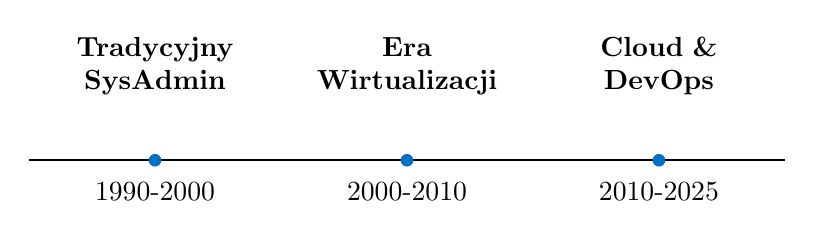
\begin{tikzpicture}[scale=0.8]
% Timeline
\draw[thick] (0,0) -- (12,0);

% Years
\node at (2,-0.5) {1990-2000};
\node at (6,-0.5) {2000-2010};
\node at (10,-0.5) {2010-2025};

% Markers
\fill[IBMBlue] (2,0) circle (0.1);
\fill[IBMBlue] (6,0) circle (0.1);
\fill[IBMBlue] (10,0) circle (0.1);

% Content boxes
\node[text width=3cm, align=center] at (2,1.5) {\textbf{Tradycyjny\\SysAdmin}};
\node[text width=3cm, align=center] at (6,1.5) {\textbf{Era\\Wirtualizacji}};
\node[text width=3cm, align=center] at (10,1.5) {\textbf{Cloud \&\\DevOps}};

\end{tikzpicture}

\vspace{0.5cm}
\begin{itemize}
\item \textbf{1990-2000:} Fizyczne serwery, reaktywne utrzymanie
\item \textbf{2000-2010:} VMware, centralne zarządzanie
\item \textbf{2010-2025:} Cloud-first, Infrastructure as Code, automatyzacja
\end{itemize}
\end{frame}

\begin{frame}{Tradycyjny model (1990-2000)}
\begin{columns}[T]
\begin{column}{0.5\textwidth}
\textbf{Charakterystyka roli:}
\begin{itemize}
\item Zarządzanie fizycznymi serwerami
\item Instalacja i konfiguracja OS
\item Backup na taśmach i płytach
\item Reaktywne rozwiązywanie problemów
\item Podział: "development vs operations"
\end{itemize}
\end{column}
\begin{column}{0.5\textwidth}
\textbf{Typowe narzędzia:}
\begin{itemize}
\item Skrypty powłoki
\item Zadania Cron
\item Monitorowanie SNMP
\item Ręczne wdrożenia
\item Dokumentacja w Excel
\end{itemize}
\end{column}
\end{columns}

\begin{alertblock}{Problem}
Brak automatyzacji, długie czasy wdrożenia, wysokie ryzyko błędów ludzkich, słaba skalowalność
\end{alertblock}
\end{frame}

\begin{frame}{Era wirtualizacji (2000-2010)}
\begin{columns}[T]
\begin{column}{0.5\textwidth}
\textbf{Wpływ VMware:}
\begin{itemize}
\item Maksymalizacja wykorzystania sprzętu
\item Łatwiejsze zarządzanie zasobami  
\item Pierwsze kroki automatyzacji
\item Scentralizowane zarządzanie (vCenter)
\end{itemize}
\end{column}
\begin{column}{0.5\textwidth}
\textbf{Nowe wyzwania:}
\begin{itemize}
\item Złożoność środowisk wirtualnych
\item Potrzeba nowych umiejętności
\item Sieciowe przechowywanie danych (SAN/NAS)
\item Kopie zapasowe maszyn wirtualnych
\end{itemize}
\end{column}
\end{columns}

\begin{block}{Kluczowa zmiana}
Przejście od zarządzania sprzętem do zarządzania abstrakcją - pierwsza lekcja Infrastructure as Code
\end{block}
\end{frame}

\begin{frame}{Rewolucja chmurowa (2010-2025)}
\begin{columns}[T]
\begin{column}{0.5\textwidth}
\textbf{Transformacja AWS/Azure/GCP:}
\begin{itemize}
\item Infrastructure as a Service (IaaS)
\item Platform as a Service (PaaS)  
\item Serverless computing
\item Pay-per-use model
\item Global scale w minuty
\end{itemize}
\end{column}
\begin{column}{0.5\textwidth}
\textbf{Nowe role:}
\begin{itemize}
\item Cloud Architect
\item DevOps Engineer
\item Site Reliability Engineer (SRE)
\item Platform Engineer
\item DevSecOps Specialist
\end{itemize}
\end{column}
\end{columns}

\begin{exampleblock}{Kluczowe zmiany umiejętności}
Od "click-click" do "code-code" - API-first approach, Infrastructure as Code, monitoring i observability
\end{exampleblock}
\end{frame}

\begin{frame}{Statystyki transformacji}
\begin{columns}[T]
\begin{column}{0.5\textwidth}
\textbf{Wzrost danych globalnych:}
\begin{itemize}
\item 2020: 64.2 ZB
\item 2025: 180 ZB (przewidywane)
\item Wzrost o 180\% w 5 lat
\end{itemize}

\textbf{Rynek chmury:}
\begin{itemize}
\item 2022: \$483B
\item 2030: \$1.6T (przewidywane)
\item CAGR: 15.7\%
\end{itemize}
\end{column}
\begin{column}{0.5\textwidth}
\textbf{Adopcja multi-cloud:}
\begin{itemize}
\item 87\% organizacji (2024)
\item Średnio 2.6 cloud providers
\item Hybrid cloud: 65\% enterprise
\end{itemize}

\textbf{Adopcja DevOps:}
\begin{itemize}
\item 83\% organizacji IT
\item 200x częstsze wdrożenia
\item 24x szybsze odzyskiwanie
\end{itemize}
\end{column}
\end{columns}
\end{frame}

% Section 3: DevOps Philosophy
\section{Podstawy filozofii DevOps}

\begin{frame}{Co to jest DevOps?}
\begin{alertblock}{Definicja}
\textbf{DevOps} = Development + Operations = metodologia skracająca cykl SDLC przy jednoczesnym zapewnieniu wysokiej jakości oprogramowania
\end{alertblock}

\begin{columns}[T]
\begin{column}{0.5\textwidth}
\textbf{Historia powstania:}
\begin{itemize}
\item 2009: Patrick Debois - "DevOpsDays" Belgia
\item John Allspaw \& Paul Hammond - "10+ Deploys Per Day" (Flickr)
\item Odpowiedź na problemy komunikacji dev-ops
\end{itemize}
\end{column}
\begin{column}{0.5\textwidth}
\textbf{Kluczowe założenia:}
\begin{itemize}
\item Szybsze dostarczanie wartości biznesowej
\item Większa niezawodność systemów
\item Redukcja ryzyka przy wdrożeniach
\item Lepsza współpraca zespołów
\end{itemize}
\end{column}
\end{columns}

\begin{block}{"You build it, you run it" - Amazon}
Zespoły deweloperskie biorą pełną odpowiedzialność za cały cykl życia aplikacji
\end{block}
\end{frame}

\begin{frame}{Framework CALMS}
\begin{center}
\Large\textbf{C.A.L.M.S}
\end{center}

\begin{columns}[T]
\begin{column}{0.2\textwidth}
\centering
\textcolor{IBMBlue}{\textbf{\Large C}}\\
\textbf{Culture}\\
\small Kultura
\end{column}
\begin{column}{0.2\textwidth}
\centering
\textcolor{IBMBlue}{\textbf{\Large A}}\\
\textbf{Automation}\\
\small Automatyzacja
\end{column}
\begin{column}{0.2\textwidth}
\centering
\textcolor{IBMBlue}{\textbf{\Large L}}\\
\textbf{Lean}\\
\small Szczupłość
\end{column}
\begin{column}{0.2\textwidth}
\centering
\textcolor{IBMBlue}{\textbf{\Large M}}\\
\textbf{Measurement}\\
\small Pomiary
\end{column}
\begin{column}{0.2\textwidth}
\centering
\textcolor{IBMBlue}{\textbf{\Large S}}\\
\textbf{Sharing}\\
\small Dzielenie się
\end{column}
\end{columns}

\vspace{1cm}
\begin{block}{Holistyczne podejście}
DevOps to nie tylko narzędzia - to transformacja kulturowa, procesowa i technologiczna jednocześnie
\end{block}
\end{frame}

\begin{frame}{C - Culture (Kultura)}
\begin{columns}[T]
\begin{column}{0.5\textwidth}
\textbf{Wspólna odpowiedzialność:}
\begin{itemize}
\item Wspólna odpowiedzialność za produkt
\item Koniec z "nie mój problem"
\item Własność od początku do końca
\end{itemize}

\textbf{Bezpieczeństwo psychologiczne:}
\begin{itemize}
\item Prawo do błędu i uczenia się
\item Analizy bez przypisywania winy
\item Kultura eksperymentowania
\end{itemize}
\end{column}
\begin{column}{0.5\textwidth}
\textbf{Łamanie silosów:}
\begin{itemize}
\item Likwidacja barier organizacyjnych
\item Zespoły międzyfunkcyjne
\item Wspólne cele i metryki
\end{itemize}

\textbf{Ciągłe uczenie się:}
\begin{itemize}
\item Inwestycja w rozwój zespołu
\item Sesje dzielenia się wiedzą
\item Społeczności praktyków
\end{itemize}
\end{column}
\end{columns}

\begin{exampleblock}{Przykład: Netflix}
"Freedom and Responsibility" culture - autonomia zespołów przy jasnych oczekiwaniach biznesowych
\end{exampleblock}
\end{frame}

\begin{frame}{A - Automation (Automatyzacja)}
\begin{columns}[T]
\begin{column}{0.5\textwidth}
\textbf{Pipelines CI/CD:}
\begin{itemize}
\item Automatyczne budowanie
\item Automatyczne testowanie
\item Automatyczne wdrażanie
\item Mechanizmy cofania zmian
\end{itemize}

\textbf{Infrastruktura jako kod:}
\begin{itemize}
\item Terraform, Ansible, Pulumi
\item Wersjonowana infrastruktura
\item Powtarzalne środowiska
\end{itemize}
\end{column}
\begin{column}{0.5\textwidth}
\textbf{Automatyzacja testów:}
\begin{itemize}
\item Testy jednostkowe
\item Testy integracyjne
\item Testy end-to-end
\item Testy wydajnościowe
\end{itemize}

\textbf{Systemy samoleczące:}
\begin{itemize}
\item Automatyczne skalowanie
\item Kontrole zdrowia
\item Automatyczne odzyskiwanie
\item Wyłączniki bezpieczeństwa
\end{itemize}
\end{column}
\end{columns}

\begin{exampleblock}{Przykład: Facebook}
1000+ wdrożeń dziennie dzięki pełnej automatyzacji potoków
\end{exampleblock}
\end{frame}

\begin{frame}{L - Lean (Szczupłość)}
\begin{columns}[T]
\begin{column}{0.5\textwidth}
\textbf{Minimalizacja marnotrawstwa:}
\begin{itemize}
\item Eliminacja marnotrawstwa
\item Skupienie na działaniach dodających wartość
\item Redukcja przełączania kontekstu
\end{itemize}

\textbf{Małe partie:}
\begin{itemize}
\item Częste, małe zmiany
\item Ograniczony zasięg błędów
\item Szybsze pętle informacji zwrotnej
\end{itemize}
\end{column}
\begin{column}{0.5\textwidth}
\textbf{Mapowanie strumienia wartości:}
\begin{itemize}
\item Optymalizacja przepływu wartości
\item Identyfikacja wąskich gardeł
\item Skrócenie czasu realizacji
\end{itemize}

\textbf{Szybko błądzić, szybko uczyć się:}
\begin{itemize}
\item Szybkie wykrywanie błędów
\item Szybkie prototypowanie
\item Iteracyjne doskonalenie
\end{itemize}
\end{column}
\end{columns}

\begin{block}{Kluczowa zasada}
Optymalizacja całego systemu, nie pojedynczych komponentów
\end{block}
\end{frame}

\begin{frame}{M - Measurement (Pomiary)}
\begin{columns}[T]
\begin{column}{0.5\textwidth}
\textbf{Metryki techniczne:}
\begin{itemize}
\item MTTR (średni czas odzyskiwania)
\item MTBF (średni czas między awariami)
\item Częstotliwość wdrożeń
\item Czas realizacji zmian
\end{itemize}

\textbf{Metryki biznesowe:}
\begin{itemize}
\item Zadowolenie klientów
\item Wpływ na przychody
\item Wskaźnik adopcji funkcji
\item Zaangażowanie użytkowników
\end{itemize}
\end{column}
\begin{column}{0.5\textwidth}
\textbf{Obserwowalność:}
\begin{itemize}
\item Metryki, logi, ślady
\item Monitorowanie w czasie rzeczywistym
\item Strategie alertów
\item Pulpity i wizualizacja
\end{itemize}

\textbf{Decyzje oparte na danych:}
\begin{itemize}
\item Testy A/B
\item Przełączniki funkcji
\item Testy porównawcze wydajności
\item Planowanie pojemności
\end{itemize}
\end{column}
\end{columns}

\begin{alertblock}{Pamiętaj}
"Nie można ulepszyć tego, czego się nie mierzy" - ciągłe monitorowanie wszystkich aspektów systemu
\end{alertblock}
\end{frame}

\begin{frame}{S - Sharing (Dzielenie się)}
\begin{columns}[T]
\begin{column}{0.5\textwidth}
\textbf{Dzielenie się wiedzą:}
\begin{itemize}
\item Dokumentacja jako kod
\item Wewnętrzne wiki i podręczniki
\item Regularne sesje szkoleniowe
\item Prezentacje techniczne
\end{itemize}

\textbf{Standaryzacja narzędzi:}
\begin{itemize}
\item Wspólne narzędzia i praktyki
\item Współdzielone biblioteki i komponenty
\item Standardowe procedury operacyjne
\end{itemize}
\end{column}
\begin{column}{0.5\textwidth}
\textbf{Zespoły międzyfunkcyjne:}
\begin{itemize}
\item Zespoły międzyfunkcyjne
\item Wbudowani inżynierowie operacyjni
\item Wspólna odpowiedzialność za dyżury
\end{itemize}

\textbf{Otwarta komunikacja:}
\begin{itemize}
\item Transparentność procesów
\item Regularne retrospektywy
\item Dzielenie się incydentami i uczenie
\end{itemize}
\end{column}
\end{columns}

\begin{block}{Community Building}
Tworzenie wewnętrznych społeczności praktyków - silosy znikają, wiedza się rozprzestrzenia
\end{block}
\end{frame}

\begin{frame}{Korzyści DevOps - dane z State of DevOps Report 2024}
\begin{columns}[T]
\begin{column}{0.5\textwidth}
\textbf{Metryki wydajności:}
\begin{itemize}
\item \textcolor{green}{\textbf{200x}} częstsze wdrożenia
\item \textcolor{green}{\textbf{24x}} szybsze odzyskiwanie po incydentach
\item \textcolor{green}{\textbf{3x}} niższa częstotliwość błędów
\item \textcolor{green}{\textbf{50\%}} mniej czasu na poprawki
\end{itemize}
\end{column}
\begin{column}{0.5\textwidth}
\textbf{Wpływ biznesowy:}
\begin{itemize}
\item \textcolor{blue}{\textbf{23\%}} wzrost rentowności
\item \textcolor{blue}{\textbf{19\%}} wzrost udziału w rynku
\item \textcolor{blue}{\textbf{18\%}} wzrost produktywności
\item \textcolor{blue}{\textbf{12\%}} wzrost zadowolenia klientów
\end{itemize}
\end{column}
\end{columns}

\vspace{1cm}
\begin{alertblock}{Elite Performers}
Najlepsze 25\% organizacji osiąga wszystkie powyższe metryki jednocześnie - DevOps jako przewaga konkurencyjna
\end{alertblock}
\end{frame}

\begin{frame}{Wyzwania implementacji DevOps}
\begin{columns}[T]
\begin{column}{0.5\textwidth}
\textbf{Organizacyjne:}
\begin{itemize}
\item \textcolor{red}{Opór kulturowy} - "zawsze tak robiliśmy"
\item \textcolor{red}{Mentalność silosów} - zachowania terytorialne
\item \textcolor{red}{Brak wsparcia kierownictwa}
\item \textcolor{red}{Niewystarczający budżet szkoleniowy}
\end{itemize}

\textbf{Techniczne:}
\begin{itemize}
\item \textcolor{orange}{Systemy dziedziczone} - dług techniczny
\item \textcolor{orange}{Rozproszenie narzędzi} - za dużo narzędzi
\item \textcolor{orange}{Obawy bezpieczeństwa} - luka DevSecOps
\end{itemize}
\end{column}
\begin{column}{0.5\textwidth}
\textbf{Anti-patterns do unikania:}
\begin{itemize}
\item "DevOps team" jako kolejne silos
\item Automatyzacja bez zmiany kultury
\item Pomijanie testów w pogoni za szybkością
\item Brak monitorowania w produkcji
\item "DevOps engineer" zamiast wspólnej odpowiedzialności
\end{itemize}
\end{column}
\end{columns}

\begin{block}{Kluczowy insight}
Transformacja DevOps = 20\% narzędzia, 80\% kultura i procesy
\end{block}
\end{frame}

% Section 4: Trendy 2025
\section{Współczesne wyzwania i trendy IT 2025}

\begin{frame}{AI/ML Revolution w IT Operations}
\begin{alertblock}{AIOps - Artificial Intelligence for IT Operations}
Zastosowanie uczenia maszynowego do automatyzacji i optymalizacji operacji IT
\end{alertblock}

\begin{columns}[T]
\begin{column}{0.5\textwidth}
\textbf{Praktyczne zastosowania:}
\begin{itemize}
\item \textbf{Analityka predykcyjna} - konserwacja zapobiegawcza
\item \textbf{Wykrywanie anomalii} - automatyczne wykrywanie incydentów
\item \textbf{Inteligentna alokacja zasobów} - optymalizacja kosztów
\item \textbf{Rozpoznawanie wzorców} - analiza logów i przyczyn źródłowych
\end{itemize}
\end{column}
\begin{column}{0.5\textwidth}
\textbf{Narzędzia i platformy:}
\begin{itemize}
\item Datadog Intelligence
\item Microsoft Azure Monitor
\item Google Cloud Operations Suite
\item Splunk IT Service Intelligence
\item Dynatrace Davis AI
\end{itemize}
\end{column}
\end{columns}

\begin{exampleblock}{Wpływ na role}
Przejście od operacji reaktywnych do predykcyjnych - nowe umiejętności: podstawy nauki o danych, interpretacja modeli ML
\end{exampleblock}
\end{frame}

\begin{frame}{Platform Engineering - nowy paradygmat}
\begin{alertblock}{Platform Engineering}
Dyscyplina projektowania i budowy łańcuchów narzędziowych i przepływów pracy, które umożliwiają samoobsługowe możliwości dla inżynierów oprogramowania w erze cloud-native
\end{alertblock}

\begin{columns}[T]
\begin{column}{0.5\textwidth}
\textbf{Wewnętrzna platforma deweloperska (IDP):}
\begin{itemize}
\item Samoobsługowa infrastruktura
\item Złote ścieżki i szablony
\item Optymalizacja doświadczenia dewelopera
\item Standardowe wzorce wdrażania
\end{itemize}
\end{column}
\begin{column}{0.5\textwidth}
\textbf{Korzyści:}
\begin{itemize}
\item Obniżone obciążenie poznawcze deweloperów
\item Szybszy czas wprowadzenia do produkcji
\item Zwiększona produktywność deweloperów
\item Spójne bezpieczeństwo i zgodność
\end{itemize}
\end{column}
\end{columns}

\begin{exampleblock}{Przykłady platform}
Spotify Backstage, Netflix Spinnaker, Uber Peloton, Google Borg
\end{exampleblock}
\end{frame}

\begin{frame}{Edge Computing i distributed infrastructure}
\begin{columns}[T]
\begin{column}{0.5\textwidth}
\textbf{Czynniki napędzające Edge Computing:}
\begin{itemize}
\item Proliferacja sieci 5G
\item Eksplozja urządzeń IoT
\item Wymagania niskich opóźnień
\item Regulacje lokalności danych (GDPR)
\item Optymalizacja kosztów przepustowości
\end{itemize}

\textbf{Wzorce architektoniczne:}
\begin{itemize}
\item Kubernetes na brzegu (k3s, MicroK8s)
\item Ewolucja CDN
\item Fog computing
\item Wielodostępowe przetwarzanie brzegowe (MEC)
\end{itemize}
\end{column}
\begin{column}{0.5\textwidth}
\textbf{Wyzwania dla administratorów:}
\begin{itemize}
\item Zarządzanie tysiącami węzłów brzegowych
\item Bezpieczeństwo w środowiskach rozproszonych
\item Monitorowanie na masową skalę
\item Niezawodność i łączność sieci
\item Automatyczne udostępnianie i aktualizacje
\end{itemize}

\textbf{Nowe umiejętności:}
\begin{itemize}
\item Platformy orkiestracji brzegowej
\item Programowanie sieciowe
\item Debugowanie systemów rozproszonych
\end{itemize}
\end{column}
\end{columns}
\end{frame}

\begin{frame}{Sustainability i Green IT}
\begin{alertblock}{Green Computing Imperative}
Europejski Zielony Ład i regulacje ESG wymuszają optymalizację śladu węglowego w operacjach IT
\end{alertblock}

\begin{columns}[T]
\begin{column}{0.5\textwidth}
\textbf{Optymalizacja śladu węglowego:}
\begin{itemize}
\item Energooszczędne planowanie obciążeń
\item Wybór zielonych regionów chmury
\item Właściwe wymiarowanie i optymalizacja zasobów  
\item Śledzenie wykorzystania energii odnawialnej
\item Narzędzia oceny cyklu życia
\end{itemize}
\end{column}
\begin{column}{0.5\textwidth}
\textbf{Praktyczne działania:}
\begin{itemize}
\item Autoskalowanie uwzględniające emisję CO2
\item Zrównoważony rozwój oprogramowania
\item Zielone pipelines CI/CD
\item Monitorowanie i raportowanie energii
\item Gospodarka cyrkularowa w sprzęcie IT
\end{itemize}
\end{column}
\end{columns}

\begin{block}{Regulatory landscape}
Taksonomia UE, Dyrektywa o raportowaniu zrównoważoności przedsiębiorstw (CSRD) - zgodność staje się obowiązkowa
\end{block}
\end{frame}

\begin{frame}{Zero Trust Security Architecture}
\begin{alertblock}{"Never trust, always verify"}
Model bezpieczeństwa oparty na ciągłej weryfikacji zamiast ochrony perymetrycznej
\end{alertblock}

\begin{columns}[T]
\begin{column}{0.5\textwidth}
\textbf{Główne zasady:}
\begin{itemize}
\item Model bezpieczeństwa zorientowany na tożsamość
\item Dostęp z najmniejszymi uprawnieniami
\item Mikrosegmentacja
\item Ciągłe uwierzytelnianie
\item Założenie naruszenia
\end{itemize}

\textbf{Obszary implementacji:}
\begin{itemize}
\item Bezpieczeństwo sieci (SASE)
\item Zarządzanie tożsamością i dostępem
\item Bezpieczeństwo urządzeń i aplikacji
\end{itemize}
\end{column}
\begin{column}{0.5\textwidth}
\textbf{Integracja DevSecOps:}
\begin{itemize}
\item Bezpieczeństwo wbudowane w CI/CD
\item Polityki jako kod
\item Automatyczne sprawdzanie zgodności
\item Automatyzacja testów bezpieczeństwa
\item Automatyzacja reakcji na incydenty
\end{itemize}

\textbf{Ekosystem narzędzi:}
\begin{itemize}
\item HashiCorp Boundary
\item Okta Workforce Identity
\item Palo Alto Prisma
\item Microsoft Conditional Access
\end{itemize}
\end{column}
\end{columns}
\end{frame}

% Section 5: Case Study
\section{Case Study: Santander Bank Polska}

\begin{frame}{Case Study: Santander Bank Polska - DevOps Transformation}
\begin{alertblock}{Context}
Transformacja DevOps w organizacji finansowej - zgodność regulacyjna + innowacje cyfrowe
\end{alertblock}

\begin{columns}[T]
\begin{column}{0.5\textwidth}
\textbf{Sytuacja wyjściowa (2012):}
\begin{itemize}
\item Dziedziczone narzędzia zarządzania projektami
\item Manualne procesy wdrażania  
\item Długie cykle wydań
\item Słaba komunikacja zespołów dev-ops
\item Wyzwania zgodności regulacyjnej
\end{itemize}
\end{column}
\begin{column}{0.5\textwidth}
\textbf{Czynniki biznesowe:}
\begin{itemize}
\item Konkurencja z fintechami
\item Oczekiwania klientów - bankowość cyfrowa
\item Wymagania regulacyjne (PCI-DSS, GDPR)
\item Presja optymalizacji kosztów
\item Przyspieszenie czasu wprowadzenia na rynek
\end{itemize}
\end{column}
\end{columns}

\begin{block}{Kluczowe wyzwanie}
Jak połączyć zwinność DevOps z surowymi wymaganiami zgodności w branży finansowej?
\end{block}
\end{frame}

\begin{frame}{Faza 1: Process Management (2012-2013)}
\begin{columns}[T]
\begin{column}{0.5\textwidth}
\textbf{Implementowane rozwiązania:}
\begin{itemize}
\item Migracja z dziedziczonych narzędzi do \textbf{Atlassian Jira}
\item Integracja z CMDB i zarządzaniem zmianami
\item Ulepszone śledzenie błędów i zarządzanie wydaniami  
\item Raportowanie online na wszystkich poziomach
\item Zautomatyzowany przepływ pracy dla zatwierdzeń
\end{itemize}
\end{column}
\begin{column}{0.5\textwidth}
\textbf{Napotkane wyzwania:}
\begin{itemize}
\item Opór użytkowników przed adopcją
\item Złożoność migracji danych
\item Integracja z istniejącymi systemami
\item Szkolenia i zarządzanie zmianą
\item Dostosowanie do procesów bankowych
\end{itemize}
\end{column}
\end{columns}

\begin{exampleblock}{Key insight}
Adopcja narzędzi bez standaryzacji procesów = ograniczony wpływ. Zmiana kultury równie ważna jak technologia.
\end{exampleblock}
\end{frame}

\begin{frame}{Faza 2: Automation (2015-2016)}
\begin{columns}[T]
\begin{column}{0.5\textwidth}
\textbf{Implementacja automatyzacji:}
\begin{itemize}
\item \textbf{JFrog Artifactory} - scentralizowane zarządzanie artefaktami
\item Zautomatyzowane pipelines wdrożeniowe
\item Integracja z \textbf{IBM UrbanCode Deploy}
\item Standaryzacja repozytoriów pakietów
\item Integracja automatycznych testów
\end{itemize}
\end{column}
\begin{column}{0.5\textwidth}
\textbf{Stos techniczny:}
\begin{itemize}
\item \textbf{Jenkins} - automatyzacja CI/CD
\item \textbf{BMC Remedy} - integracja zarządzania zmianami
\item Niestandardowe skrypty do wdrożeń
\item Automatyzacja migracji baz danych
\item Automatyzacja udostępniania środowisk
\end{itemize}
\end{column}
\end{columns}

\begin{block}{Banking-specific considerations}
Automatyczne ślady audytu, procedury cofania, przepływy zatwierdzeń regulacyjnych - automatyzacja zgodności
\end{block}
\end{frame}


\begin{frame}{Rezultaty i wnioski}
\begin{columns}[T]
\begin{column}{0.5\textwidth}
\textbf{Osiągnięte korzyści:}
\begin{itemize}
\item \textcolor{green}{\textbf{70\%}} skrócenie czasu wdrożenia
\item \textcolor{green}{\textbf{Poprawiona}} stabilność systemu
\item \textcolor{green}{\textbf{Lepsza}} śledzalność i zgodność
\item \textcolor{green}{\textbf{Większa}} współpraca zespołowa
\item \textcolor{green}{\textbf{Mniej}} błędów manualnych
\end{itemize}
\end{column}
\begin{column}{0.5\textwidth}
\textbf{Kluczowe czynniki sukcesu:}
\begin{itemize}
\item \textbf{Wsparcie zarządu} - zaangażowanie kadry kierowniczej
\item \textbf{Podejście stopniowe} - wdrożenie etapami
\item \textbf{Inwestycja w szkolenia} - rozwój kompetencji zespołu
\item \textbf{Najpierw optymalizacja, potem automatyzacja}
\item \textbf{Integracja zgodności} - bezpieczeństwo od początku
\end{itemize}
\end{column}
\end{columns}

\begin{alertblock}{Critical lesson}
W branży finansowej: zgodność nie jest ograniczeniem dla DevOps - to wymaganie, które może być zautomatyzowane
\end{alertblock}
\end{frame}

\begin{frame}{Uniwersalne wnioski dla polskich firm}
\begin{block}{Co się sprawdza w polskim kontekście?}
\begin{itemize}
\item \textbf{Stopniowa transformacja} - nie podejście "big bang"
\item \textbf{Rozwiązania hybrydowe} - integracja z systemami dziedziczonymi
\item \textbf{Mentalność zgodności na pierwszym miejscu} - szczególnie w regulowanych branżach  
\item \textbf{Inwestycja w szkolenia zespołów} - przekwalifikowanie istniejącej kadry
\item \textbf{Standaryzacja narzędzi} - redukcja złożoności, poprawa utrzymywalności
\end{itemize}
\end{block}

\begin{exampleblock}{Inne polskie historie sukcesu}
\begin{itemize}
\item \textbf{Allegro} - transformacja mikroserwisów na Kubernetes
\item \textbf{CD Projekt} - pipelines CI/CD w tworzeniu gier
\item \textbf{Asseco} - inżynieria platform dla klientów finansowych
\end{itemize}
\end{exampleblock}
\end{frame}

% Section 6: Summary
\section{Podsumowanie}

\begin{frame}{Kluczowe wnioski z wykładu}
\begin{alertblock}{1. Rola administratora ewoluuje}
Od reaktywnego utrzymania do proaktywnej inżynierii - Infrastruktura jako kod, myślenie automation-first
\end{alertblock}

\begin{block}{2. DevOps to kultura, nie narzędzia}
CALMS framework jako przewodnik transformacji - Culture, Automation, Lean, Measurement, Sharing
\end{block}

\begin{exampleblock}{3. AI i automatyzacja zmieniają landscape}
AIOps, Platform Engineering, Edge Computing - nowe umiejętności są kluczowe dla rozwoju kariery
\end{exampleblock}

\begin{alertblock}{4. Polskie firmy skutecznie implementują DevOps}
Santander, Allegro - przykłady do naśladowania, skupienie na zgodności i podejściu stopniowym
\end{alertblock}
\end{frame}

\begin{frame}{Następne kroki w kursie}
\begin{columns}[T]
\begin{column}{0.5\textwidth}
\textbf{Wykład 2 (następny tydzień):}
\begin{itemize}
\item \textbf{Konteneryzacja} - Docker fundamenty
\item Nowoczesne praktyki 2025
\item Bezpieczeństwo kontenerów
\item Budowy wieloetapowe
\item Alternatywy: Podman, containerd
\end{itemize}
\end{column}
\begin{column}{0.5\textwidth}
\textbf{Zalecana lektura:}
\begin{itemize}
\item "The Phoenix Project" - rozdziały 1-5
\item State of DevOps Report 2024 - streszczenie kierownicze
\item Przewodnik najlepszych praktyk Docker
\item CNCF Landscape overview
\end{itemize}
\end{column}
\end{columns}
\end{frame}

\begin{frame}{Kontakt i zasoby}
\begin{columns}[T]
\begin{column}{0.5\textwidth}
\textbf{Prowadzący:}\\
\textbf{mgr inż. Jakub Woźniak}\\


\vspace{0.5cm}
\textbf{Kontakt:}\\
\href{mailto:jakub.wozniak@cs.put.poznan.pl}{jakub.wozniak@cs.put.poznan.pl}\\
\href{https://www.cs.put.poznan.pl/jwozniak}{www.cs.put.poznan.pl/jwozniak}
\end{column}
\begin{column}{0.5\textwidth}
\textbf{Dodatkowe zasoby:}
\begin{itemize}
\item CNCF Landscape: landscape.cncf.io
\item State of DevOps Reports
\item Kubernetes Documentation
\item Docker Best Practices Guide
\item AWS/Azure/GCP Documentation
\end{itemize}

\vspace{0.5cm}
\textbf{Community:}
\begin{itemize}
\item DevOps Poland Meetup
\item Kubernetes Poland
\item Cloud Native Computing Foundation
\end{itemize}
\end{column}
\end{columns}
\end{frame}

\begin{frame}
\centering
\Huge Dziękuję za uwagę!

\vspace{2cm}
\Large Pytania?

\vspace{1cm}
\normalsize
\textbf{Jakub Woźniak}\\
\href{mailto:jakub.wozniak@cs.put.poznan.pl}{jakub.wozniak@cs.put.poznan.pl}
\end{frame}

\end{document}
